% this file is called up by thesis.tex
% content in this file will be fed into the main document

\chapter{Network Design}

\section{Overview}

Chapter 4 discusses the network design of the HCMP Player.  
I focus on illustrating the design decisions behind the network function of    
the HCMP Player. A full description of network API will be provided. All other
HCMP components can communicate with the HCMP Player through the network,
with the network API. Chapter 4 also discusses how the HCMP player 
creates a connection with remote server. The implementation 
use Zeromq \cite{zeromq} library to facilitate network development. The Zeromq library 
integrates several different ways to communicate between nodes on a network.
We will briefly cover each method, together with its pros and cons, and 
its usage inside the HCMP Player.

\section{Conductor and Player}
In network module of the HCMP Player, three design patterns are used. The 
request and reply design pattern is the most common and is used to 
build the connection between remote server and the HCMP Player. 
After connection has been established, the remote server and
the HCMP Player will adopt observer pattern. 

\subsection{Request \& Reply Pattern}
The request and reply pattern is the most basic pattern used in network 
communication. Just as its name suggests the client sends request to the server,
the server receives, then handles the request and sends a reply to
the client. This pattern is heavily used in the remote procedure call (RPC) 
programming model. The caller object can invoke a method from the called 
object, whether the called object is stored in local machine memory or
in the remote machine's memory. The request and reply pattern is commonly used
in web programming. For example when a user presses a button, this event will 
invoke a method on the server. After some computation the server replies with 
a result sent to the web page. In most cases, the request and reply pattern
uses TCP to reliably deliver the message. 

Figure 4.1 indicates how the request and reply pattern is used by the HCMP Player. 
When the user tries to establish a connection with the remote server, the HCMP Player 
will send a request and wait for a reply. A timeout limit is set to 
avoid waiting too long. If the attempt to connect fails the HCMP Player
will ``rollback'' to stand-alone mode.
\begin{figure}[H]
\center{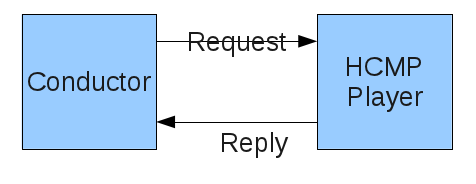
\includegraphics[width=0.55\linewidth]{4/3.png}}
\caption{Request-Reply Pattern}
\end{figure}

\subsection{Observer Pattern}
In the observer pattern, the subject object maintains a list of its 
dependents, called observers, and notifies them automatically of 
any state changes, usually by calling one of their methods.
\begin{figure}[H]
\center{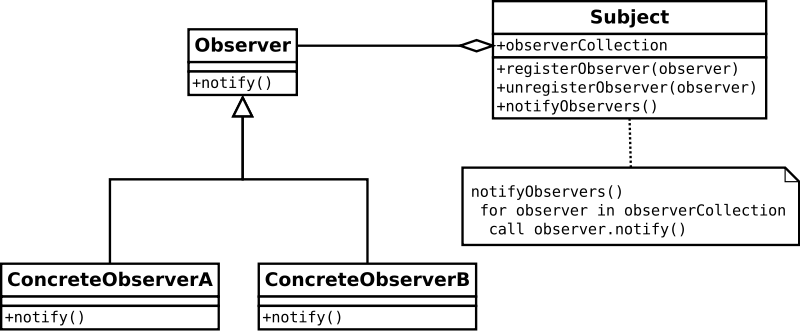
\includegraphics[width=0.8\linewidth]{4/5.png}}
\caption{UML Diagram of Observer Pattern}
\end{figure}

After a connection has been built, the Conductor and the HCMP Player form an 
observer-pattern relationship. The Conductor is the subject and the HCMP Player 
is its dependent, an observer. The HCMP Player first uses an RPC call to register 
itself in the Conductor dependents list then it waits for a reply from the Conductor. 
The conductor is responsible for synchronizing all the HCMP Players. Each Conductor 
will maintain a list of HCMP Players. This list is updated when an old player becomes 
obsolete, or a new player is created and sends an RPC call to the Conductor.
Figure 4.3 illustrates the observer pattern in HCMP Player.  
\begin{figure}[H]
\center{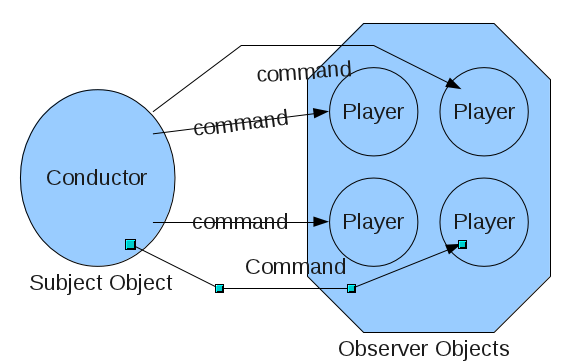
\includegraphics[width=0.65\linewidth]{4/2.png}}
\caption{Observer Pattern}
\end{figure}

\subsection{Push \& Pull Pattern}
In order to monitor the status of each HCMP Player, each registered HCMP Player 
will periodically push ``heart beat'' message to the Conductor.
The Conductor sets a count down timer for each HCMP Player it is currently 
connected to. It then periodically pulls a message and resets according to the 
HCMP Player's timer. If a timer reaches zero the Conductor will send a confirm 
message to temporarily de-register this HCMP Player from its dependent list. 
Figure 4.4 illustrates a push \& pull pattern used in HCMP Player.

\begin{figure}[H]
\center{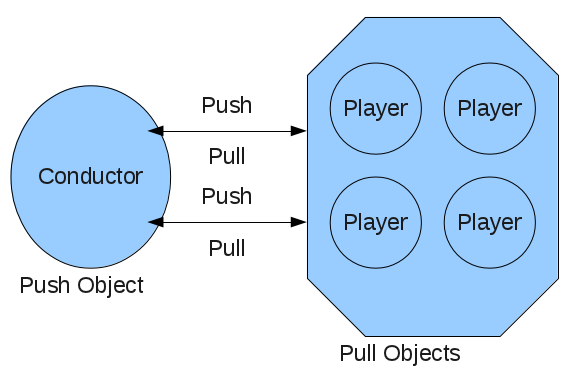
\includegraphics[width=0.65\linewidth]{4/4.png}}
\caption{Push \& Pull Pattern}
\end{figure}

\section{Network Programming Interface}
The programming interface defined below is used for communication 
between the Conductor and the HCMP Player. Any external exponent that  
uses these APIs is able to communicate with and take control of the 
HCMP Player. The GUI component is responsible for receiving all 
network request. Imagine a situation where the Conductor 
tries to take command of all the HCMP players. The Conductor sends a start
request to all HCMP players in its dependents list.
Once the request is successfully delivered, the GUI of the HCMP player will 
receive and handle the requests. After parsing the request string, 
it maps and invokes the internal command, then sends the request to the player 
engine through a message queue. The player engine reads the message queue and
schedules the first MIDI note, and the HCMP Player begins to play.

\begin{figure}[H]
\center{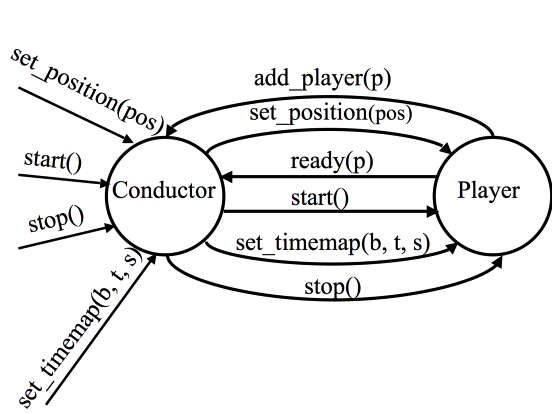
\includegraphics[width=0.5\linewidth]{3/1.png}}
\caption{HCMP Player Network API \cite{Dawen:2011}}
\end{figure}
Figure 4.5 illustrate how conductor coordinates with the HCMP Player, all the  
related commands are list below \\

From Conductor to HCMP Player
\begin{itemize}
  \item \texttt{play - start playing}  
  \item \texttt{stop - stop playing}
  \item \texttt{pause - pause current playing}
  \item \texttt{update\_time\_map - send new time map to player}  
  \item \texttt{set\_position - set play position to the given parameter}
\end{itemize}

From HCMP Player to Conductor 
\begin{itemize}
  \item \texttt{play\_all - inform the remote server to play}  
  \item \texttt{stop\_all - inform the remote server to stop}  
  \item \texttt{ready - inform the remote server is ready to play}
  \item \texttt{position - inform remote server to begin from specified position}
\end{itemize}
